\documentclass[1p]{elsarticle_modified}
%\bibliographystyle{elsarticle-num}

%\usepackage[colorlinks]{hyperref}
%\usepackage{abbrmath_seonhwa} %\Abb, \Ascr, \Acal ,\Abf, \Afrak
\usepackage{amsfonts}
\usepackage{amssymb}
\usepackage{amsmath}
\usepackage{amsthm}
\usepackage{scalefnt}
\usepackage{amsbsy}
\usepackage{kotex}
\usepackage{caption}
\usepackage{subfig}
\usepackage{color}
\usepackage{graphicx}
\usepackage{xcolor} %% white, black, red, green, blue, cyan, magenta, yellow
\usepackage{float}
\usepackage{setspace}
\usepackage{hyperref}

\usepackage{tikz}
\usetikzlibrary{arrows}

\usepackage{multirow}
\usepackage{array} % fixed length table
\usepackage{hhline}

%%%%%%%%%%%%%%%%%%%%%
\makeatletter
\renewcommand*\env@matrix[1][\arraystretch]{%
	\edef\arraystretch{#1}%
	\hskip -\arraycolsep
	\let\@ifnextchar\new@ifnextchar
	\array{*\c@MaxMatrixCols c}}
\makeatother %https://tex.stackexchange.com/questions/14071/how-can-i-increase-the-line-spacing-in-a-matrix
%%%%%%%%%%%%%%%

\usepackage[normalem]{ulem}

\newcommand{\msout}[1]{\ifmmode\text{\sout{\ensuremath{#1}}}\else\sout{#1}\fi}
%SOURCE: \msout is \stkout macro in https://tex.stackexchange.com/questions/20609/strikeout-in-math-mode

\newcommand{\cancel}[1]{
	\ifmmode
	{\color{red}\msout{#1}}
	\else
	{\color{red}\sout{#1}}
	\fi
}

\newcommand{\add}[1]{
	{\color{blue}\uwave{#1}}
}

\newcommand{\replace}[2]{
	\ifmmode
	{\color{red}\msout{#1}}{\color{blue}\uwave{#2}}
	\else
	{\color{red}\sout{#1}}{\color{blue}\uwave{#2}}
	\fi
}

\newcommand{\Sol}{\mathcal{S}} %segment
\newcommand{\D}{D} %diagram
\newcommand{\A}{\mathcal{A}} %arc


%%%%%%%%%%%%%%%%%%%%%%%%%%%%%5 test

\def\sl{\operatorname{\textup{SL}}(2,\Cbb)}
\def\psl{\operatorname{\textup{PSL}}(2,\Cbb)}
\def\quan{\mkern 1mu \triangleright \mkern 1mu}

\theoremstyle{definition}
\newtheorem{thm}{Theorem}[section]
\newtheorem{prop}[thm]{Proposition}
\newtheorem{lem}[thm]{Lemma}
\newtheorem{ques}[thm]{Question}
\newtheorem{cor}[thm]{Corollary}
\newtheorem{defn}[thm]{Definition}
\newtheorem{exam}[thm]{Example}
\newtheorem{rmk}[thm]{Remark}
\newtheorem{alg}[thm]{Algorithm}

\newcommand{\I}{\sqrt{-1}}
\begin{document}

%\begin{frontmatter}
%
%\title{Boundary parabolic representations of knots up to 8 crossings}
%
%%% Group authors per affiliation:
%\author{Yunhi Cho} 
%\address{Department of Mathematics, University of Seoul, Seoul, Korea}
%\ead{yhcho@uos.ac.kr}
%
%
%\author{Seonhwa Kim} %\fnref{s_kim}}
%\address{Center for Geometry and Physics, Institute for Basic Science, Pohang, 37673, Korea}
%\ead{ryeona17@ibs.re.kr}
%
%\author{Hyuk Kim}
%\address{Department of Mathematical Sciences, Seoul National University, Seoul 08826, Korea}
%\ead{hyukkim@snu.ac.kr}
%
%\author{Seokbeom Yoon}
%\address{Department of Mathematical Sciences, Seoul National University, Seoul, 08826,  Korea}
%\ead{sbyoon15@snu.ac.kr}
%
%\begin{abstract}
%We find all boundary parabolic representation of knots up to 8 crossings.
%
%\end{abstract}
%\begin{keyword}
%    \MSC[2010] 57M25 
%\end{keyword}
%
%\end{frontmatter}

%\linenumbers
%\tableofcontents
%
\newcommand\colored[1]{\textcolor{white}{\rule[-0.35ex]{0.8em}{1.4ex}}\kern-0.8em\color{red} #1}%
%\newcommand\colored[1]{\textcolor{white}{ #1}\kern-2.17ex	\textcolor{white}{ #1}\kern-1.81ex	\textcolor{white}{ #1}\kern-2.15ex\color{red}#1	}

{\Large $\underline{12a_{1192}~(K12a_{1192})}$}

\setlength{\tabcolsep}{10pt}
\renewcommand{\arraystretch}{1.6}
\vspace{1cm}\begin{tabular}{m{100pt}>{\centering\arraybackslash}m{274pt}}
\multirow{5}{120pt}{
	\centering
	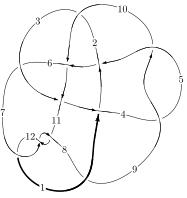
\includegraphics[width=112pt]{../../../GIT/diagram.site/Diagrams/png/1993_12a_1192.png}\\
\ \ \ A knot diagram\footnotemark}&
\allowdisplaybreaks
\textbf{Linearized knot diagam} \\
\cline{2-2}
 &
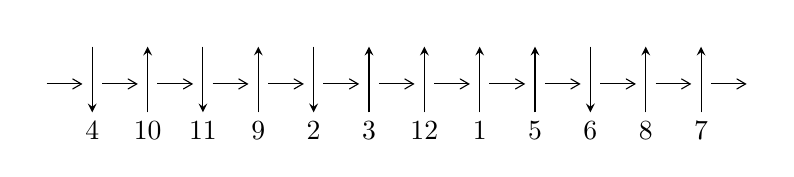
\begin{tikzpicture}[x=20pt, y=17pt]
	% nodes
	\node (C0) at (0, 0) {};
	\node (C1) at (1, 0) {};
	\node (C1U) at (1, +1) {};
	\node (C1D) at (1, -1) {4};

	\node (C2) at (2, 0) {};
	\node (C2U) at (2, +1) {};
	\node (C2D) at (2, -1) {10};

	\node (C3) at (3, 0) {};
	\node (C3U) at (3, +1) {};
	\node (C3D) at (3, -1) {11};

	\node (C4) at (4, 0) {};
	\node (C4U) at (4, +1) {};
	\node (C4D) at (4, -1) {9};

	\node (C5) at (5, 0) {};
	\node (C5U) at (5, +1) {};
	\node (C5D) at (5, -1) {2};

	\node (C6) at (6, 0) {};
	\node (C6U) at (6, +1) {};
	\node (C6D) at (6, -1) {3};

	\node (C7) at (7, 0) {};
	\node (C7U) at (7, +1) {};
	\node (C7D) at (7, -1) {12};

	\node (C8) at (8, 0) {};
	\node (C8U) at (8, +1) {};
	\node (C8D) at (8, -1) {1};

	\node (C9) at (9, 0) {};
	\node (C9U) at (9, +1) {};
	\node (C9D) at (9, -1) {5};

	\node (C10) at (10, 0) {};
	\node (C10U) at (10, +1) {};
	\node (C10D) at (10, -1) {6};

	\node (C11) at (11, 0) {};
	\node (C11U) at (11, +1) {};
	\node (C11D) at (11, -1) {8};

	\node (C12) at (12, 0) {};
	\node (C12U) at (12, +1) {};
	\node (C12D) at (12, -1) {7};
	\node (C13) at (13, 0) {};

	% arrows
	\draw[->,>={angle 60}]
	(C0) edge (C1) (C1) edge (C2) (C2) edge (C3) (C3) edge (C4) (C4) edge (C5) (C5) edge (C6) (C6) edge (C7) (C7) edge (C8) (C8) edge (C9) (C9) edge (C10) (C10) edge (C11) (C11) edge (C12) (C12) edge (C13) ;	\draw[->,>=stealth]
	(C1U) edge (C1D) (C2D) edge (C2U) (C3U) edge (C3D) (C4D) edge (C4U) (C5U) edge (C5D) (C6D) edge (C6U) (C7D) edge (C7U) (C8D) edge (C8U) (C9D) edge (C9U) (C10U) edge (C10D) (C11D) edge (C11U) (C12D) edge (C12U) ;
	\end{tikzpicture} \\
\hhline{~~} \\& 
\textbf{Solving Sequence} \\ \cline{2-2} 
 &
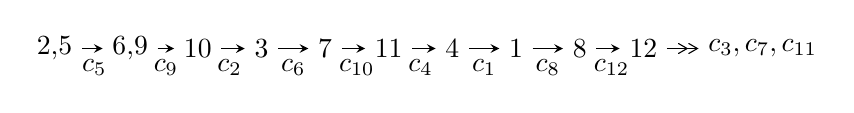
\begin{tikzpicture}[x=23pt, y=7pt]
	% node
	\node (A0) at (-1/8, 0) {2,5};
	\node (A1) at (17/16, 0) {6,9};
	\node (A2) at (17/8, 0) {10};
	\node (A3) at (25/8, 0) {3};
	\node (A4) at (33/8, 0) {7};
	\node (A5) at (41/8, 0) {11};
	\node (A6) at (49/8, 0) {4};
	\node (A7) at (57/8, 0) {1};
	\node (A8) at (65/8, 0) {8};
	\node (A9) at (73/8, 0) {12};
	\node (C1) at (1/2, -1) {$c_{5}$};
	\node (C2) at (13/8, -1) {$c_{9}$};
	\node (C3) at (21/8, -1) {$c_{2}$};
	\node (C4) at (29/8, -1) {$c_{6}$};
	\node (C5) at (37/8, -1) {$c_{10}$};
	\node (C6) at (45/8, -1) {$c_{4}$};
	\node (C7) at (53/8, -1) {$c_{1}$};
	\node (C8) at (61/8, -1) {$c_{8}$};
	\node (C9) at (69/8, -1) {$c_{12}$};
	\node (A10) at (11, 0) {$c_{3},c_{7},c_{11}$};

	% edge
	\draw[->,>=stealth]	
	(A0) edge (A1) (A1) edge (A2) (A2) edge (A3) (A3) edge (A4) (A4) edge (A5) (A5) edge (A6) (A6) edge (A7) (A7) edge (A8) (A8) edge (A9) ;
	\draw[->>,>={angle 60}]	
	(A9) edge (A10);
\end{tikzpicture} \\ 

\end{tabular} \\

\footnotetext{
The image of knot diagram is generated by the software ``\textbf{Draw programme}" developed by Andrew Bartholomew(\url{http://www.layer8.co.uk/maths/draw/index.htm\#Running-draw}), where we modified some parts for our purpose(\url{https://github.com/CATsTAILs/LinksPainter}).
}\phantom \\ \newline 
\centering \textbf{Ideals for irreducible components\footnotemark of $X_{\text{par}}$} 
 
\begin{align*}
I^u_{1}&=\langle 
-3.14046\times10^{797} u^{134}+7.10704\times10^{797} u^{133}+\cdots+1.10208\times10^{791} b+1.52232\times10^{797},\\
\phantom{I^u_{1}}&\phantom{= \langle  }2.52302\times10^{798} u^{134}-6.68142\times10^{798} u^{133}+\cdots+1.10208\times10^{791} a+4.59952\times10^{798},\\
\phantom{I^u_{1}}&\phantom{= \langle  }u^{135}-3 u^{134}+\cdots+34 u-1\rangle \\
I^u_{2}&=\langle 
226464710 u^{21}-557699915 u^{20}+\cdots+334625059 b+512910644,\\
\phantom{I^u_{2}}&\phantom{= \langle  }985188919589906 u^{21}-1767028920893903 u^{20}+\cdots+2608796188599443 a+5274270817374945,\\
\phantom{I^u_{2}}&\phantom{= \langle  }u^{22}-2 u^{21}+\cdots+7 u+1\rangle \\
\\
\end{align*}
\raggedright * 2 irreducible components of $\dim_{\mathbb{C}}=0$, with total 157 representations.\\
\footnotetext{All coefficients of polynomials are rational numbers. But the coefficients are sometimes approximated in decimal forms when there is not enough margin.}
\newpage
\renewcommand{\arraystretch}{1}
\centering \section*{I. $I^u_{1}= \langle -3.14\times10^{797} u^{134}+7.11\times10^{797} u^{133}+\cdots+1.10\times10^{791} b+1.52\times10^{797},\;2.52\times10^{798} u^{134}-6.68\times10^{798} u^{133}+\cdots+1.10\times10^{791} a+4.60\times10^{798},\;u^{135}-3 u^{134}+\cdots+34 u-1 \rangle$}
\flushleft \textbf{(i) Arc colorings}\\
\begin{tabular}{m{7pt} m{180pt} m{7pt} m{180pt} }
\flushright $a_{2}=$&$\begin{pmatrix}0\\u\end{pmatrix}$ \\
\flushright $a_{5}=$&$\begin{pmatrix}1\\0\end{pmatrix}$ \\
\flushright $a_{6}=$&$\begin{pmatrix}1\\u^2\end{pmatrix}$ \\
\flushright $a_{9}=$&$\begin{pmatrix}-2.28932\times10^{7} u^{134}+6.06254\times10^{7} u^{133}+\cdots+1.39248\times10^{9} u-4.17348\times10^{7}\\2.84957\times10^{6} u^{134}-6.44874\times10^{6} u^{133}+\cdots+2.44178\times10^{7} u-1.38132\times10^{6}\end{pmatrix}$ \\
\flushright $a_{10}=$&$\begin{pmatrix}-2.00436\times10^{7} u^{134}+5.41767\times10^{7} u^{133}+\cdots+1.41690\times10^{9} u-4.31162\times10^{7}\\2.84957\times10^{6} u^{134}-6.44874\times10^{6} u^{133}+\cdots+2.44178\times10^{7} u-1.38132\times10^{6}\end{pmatrix}$ \\
\flushright $a_{3}=$&$\begin{pmatrix}773762. u^{134}-2.08084\times10^{6} u^{133}+\cdots-6.02914\times10^{7} u+1.86749\times10^{6}\\-178328. u^{134}+397315. u^{133}+\cdots+4.37900\times10^{6} u-122221.\end{pmatrix}$ \\
\flushright $a_{7}=$&$\begin{pmatrix}-626624. u^{134}+1.63753\times10^{6} u^{133}+\cdots+2.75411\times10^{7} u-759619.\\88780.4 u^{134}-129429. u^{133}+\cdots+5.71635\times10^{6} u-194638.\end{pmatrix}$ \\
\flushright $a_{11}=$&$\begin{pmatrix}-2.34698\times10^{7} u^{134}+6.29580\times10^{7} u^{133}+\cdots+1.57488\times10^{9} u-4.76890\times10^{7}\\2.42821\times10^{6} u^{134}-5.21868\times10^{6} u^{133}+\cdots+7.18985\times10^{7} u-2.87858\times10^{6}\end{pmatrix}$ \\
\flushright $a_{4}=$&$\begin{pmatrix}145988. u^{134}-489201. u^{133}+\cdots-2.54112\times10^{7} u+819242.\\-268209. u^{134}+677536. u^{133}+\cdots+1.88772\times10^{7} u-595757.\end{pmatrix}$ \\
\flushright $a_{1}=$&$\begin{pmatrix}789912. u^{134}-2.02803\times10^{6} u^{133}+\cdots-3.64636\times10^{7} u+1.03824\times10^{6}\\18138.2 u^{134}-140403. u^{133}+\cdots-1.35309\times10^{7} u+443060.\end{pmatrix}$ \\
\flushright $a_{8}=$&$\begin{pmatrix}2.40816\times10^{7} u^{134}-6.99553\times10^{7} u^{133}+\cdots-2.52277\times10^{9} u+7.88766\times10^{7}\\-7.24295\times10^{6} u^{134}+1.86957\times10^{7} u^{133}+\cdots+3.49936\times10^{8} u-1.01956\times10^{7}\end{pmatrix}$ \\
\flushright $a_{12}=$&$\begin{pmatrix}-8.35142\times10^{6} u^{134}+2.38578\times10^{7} u^{133}+\cdots+9.08734\times10^{8} u-2.87215\times10^{7}\\1.60252\times10^{6} u^{134}-4.07114\times10^{6} u^{133}+\cdots-5.89469\times10^{7} u+1.59194\times10^{6}\end{pmatrix}$\\&\end{tabular}
\flushleft \textbf{(ii) Obstruction class $= -1$}\\~\\
\flushleft \textbf{(iii) Cusp Shapes $= 1.04402\times10^{7} u^{134}-2.72921\times10^{7} u^{133}+\cdots-5.20718\times10^{8} u+1.50984\times10^{7}$}\\~\\
\newpage\renewcommand{\arraystretch}{1}
\flushleft \textbf{(iv) u-Polynomials at the component}\newline \\
\begin{tabular}{m{50pt}|m{274pt}}
Crossings & \hspace{64pt}u-Polynomials at each crossing \\
\hline $$\begin{aligned}c_{1}\end{aligned}$$&$\begin{aligned}
&u^{135}+2 u^{134}+\cdots-28271 u-1457
\end{aligned}$\\
\hline $$\begin{aligned}c_{2}\end{aligned}$$&$\begin{aligned}
&u^{135}+3 u^{134}+\cdots-10011 u+2809
\end{aligned}$\\
\hline $$\begin{aligned}c_{3}\end{aligned}$$&$\begin{aligned}
&u^{135}+u^{133}+\cdots+378 u-49
\end{aligned}$\\
\hline $$\begin{aligned}c_{4},c_{9}\end{aligned}$$&$\begin{aligned}
&u^{135}-50 u^{133}+\cdots+1400 u+449
\end{aligned}$\\
\hline $$\begin{aligned}c_{5}\end{aligned}$$&$\begin{aligned}
&u^{135}-3 u^{134}+\cdots+34 u-1
\end{aligned}$\\
\hline $$\begin{aligned}c_{6}\end{aligned}$$&$\begin{aligned}
&u^{135}-4 u^{134}+\cdots-9766 u-1789
\end{aligned}$\\
\hline $$\begin{aligned}c_{7},c_{11},c_{12}\end{aligned}$$&$\begin{aligned}
&u^{135}+58 u^{133}+\cdots- u+1
\end{aligned}$\\
\hline $$\begin{aligned}c_{8}\end{aligned}$$&$\begin{aligned}
&u^{135}-27 u^{133}+\cdots-18053 u+20329
\end{aligned}$\\
\hline $$\begin{aligned}c_{10}\end{aligned}$$&$\begin{aligned}
&u^{135}-3 u^{134}+\cdots-274 u+31
\end{aligned}$\\
\hline
\end{tabular}\\~\\
\newpage\renewcommand{\arraystretch}{1}
\flushleft \textbf{(v) Riley Polynomials at the component}\newline \\
\begin{tabular}{m{50pt}|m{274pt}}
Crossings & \hspace{64pt}Riley Polynomials at each crossing \\
\hline $$\begin{aligned}c_{1}\end{aligned}$$&$\begin{aligned}
&y^{135}+34 y^{134}+\cdots+1958158897 y-2122849
\end{aligned}$\\
\hline $$\begin{aligned}c_{2}\end{aligned}$$&$\begin{aligned}
&y^{135}-33 y^{134}+\cdots+545632015 y-7890481
\end{aligned}$\\
\hline $$\begin{aligned}c_{3}\end{aligned}$$&$\begin{aligned}
&y^{135}+2 y^{134}+\cdots+38416 y-2401
\end{aligned}$\\
\hline $$\begin{aligned}c_{4},c_{9}\end{aligned}$$&$\begin{aligned}
&y^{135}-100 y^{134}+\cdots-1149774 y-201601
\end{aligned}$\\
\hline $$\begin{aligned}c_{5}\end{aligned}$$&$\begin{aligned}
&y^{135}+13 y^{134}+\cdots+52 y-1
\end{aligned}$\\
\hline $$\begin{aligned}c_{6}\end{aligned}$$&$\begin{aligned}
&y^{135}-18 y^{134}+\cdots+159785912 y-3200521
\end{aligned}$\\
\hline $$\begin{aligned}c_{7},c_{11},c_{12}\end{aligned}$$&$\begin{aligned}
&y^{135}+116 y^{134}+\cdots+173 y-1
\end{aligned}$\\
\hline $$\begin{aligned}c_{8}\end{aligned}$$&$\begin{aligned}
&y^{135}-54 y^{134}+\cdots+68531901341 y-413268241
\end{aligned}$\\
\hline $$\begin{aligned}c_{10}\end{aligned}$$&$\begin{aligned}
&y^{135}-15 y^{134}+\cdots+84314 y-961
\end{aligned}$\\
\hline
\end{tabular}\\~\\
\newpage\flushleft \textbf{(vi) Complex Volumes and Cusp Shapes}
$$\begin{array}{c|c|c}  
\text{Solutions to }I^u_{1}& \I (\text{vol} + \sqrt{-1}CS) & \text{Cusp shape}\\
 \hline 
\begin{aligned}
u &= \phantom{-}0.113265 + 0.987669 I \\
a &= \phantom{-}0.681297 - 0.821913 I \\
b &= \phantom{-}0.117752 + 0.128516 I\end{aligned}
 & \phantom{-}2.85172 + 4.49757 I & \phantom{-0.000000 } 0 \\ \hline\begin{aligned}
u &= \phantom{-}0.113265 - 0.987669 I \\
a &= \phantom{-}0.681297 + 0.821913 I \\
b &= \phantom{-}0.117752 - 0.128516 I\end{aligned}
 & \phantom{-}2.85172 - 4.49757 I & \phantom{-0.000000 } 0 \\ \hline\begin{aligned}
u &= \phantom{-}0.860645 + 0.535066 I \\
a &= \phantom{-}0.441767 + 0.703810 I \\
b &= -1.340190 - 0.049080 I\end{aligned}
 & \phantom{-}7.03467 + 0.12261 I & \phantom{-0.000000 } 0 \\ \hline\begin{aligned}
u &= \phantom{-}0.860645 - 0.535066 I \\
a &= \phantom{-}0.441767 - 0.703810 I \\
b &= -1.340190 + 0.049080 I\end{aligned}
 & \phantom{-}7.03467 - 0.12261 I & \phantom{-0.000000 } 0 \\ \hline\begin{aligned}
u &= \phantom{-}0.735782 + 0.648575 I \\
a &= \phantom{-}0.980427 + 0.139573 I \\
b &= -0.760865 - 0.699325 I\end{aligned}
 & -4.21596 + 3.62972 I & \phantom{-0.000000 } 0 \\ \hline\begin{aligned}
u &= \phantom{-}0.735782 - 0.648575 I \\
a &= \phantom{-}0.980427 - 0.139573 I \\
b &= -0.760865 + 0.699325 I\end{aligned}
 & -4.21596 - 3.62972 I & \phantom{-0.000000 } 0 \\ \hline\begin{aligned}
u &= \phantom{-}0.814772 + 0.641752 I \\
a &= \phantom{-}0.470909 - 0.439347 I \\
b &= -0.016937 - 0.591112 I\end{aligned}
 & -1.19670 - 4.78867 I & \phantom{-0.000000 } 0 \\ \hline\begin{aligned}
u &= \phantom{-}0.814772 - 0.641752 I \\
a &= \phantom{-}0.470909 + 0.439347 I \\
b &= -0.016937 + 0.591112 I\end{aligned}
 & -1.19670 + 4.78867 I & \phantom{-0.000000 } 0 \\ \hline\begin{aligned}
u &= -1.037490 + 0.121745 I \\
a &= \phantom{-}0.664354 + 0.132282 I \\
b &= \phantom{-}0.680662 - 0.447198 I\end{aligned}
 & -7.16367 - 0.20216 I & \phantom{-0.000000 } 0 \\ \hline\begin{aligned}
u &= -1.037490 - 0.121745 I \\
a &= \phantom{-}0.664354 - 0.132282 I \\
b &= \phantom{-}0.680662 + 0.447198 I\end{aligned}
 & -7.16367 + 0.20216 I & \phantom{-0.000000 } 0\\
 \hline 
 \end{array}$$\newpage$$\begin{array}{c|c|c}  
\text{Solutions to }I^u_{1}& \I (\text{vol} + \sqrt{-1}CS) & \text{Cusp shape}\\
 \hline 
\begin{aligned}
u &= -1.025180 + 0.259325 I \\
a &= -0.259943 - 0.174105 I \\
b &= -0.143730 - 0.472481 I\end{aligned}
 & -2.40598 + 0.14159 I & \phantom{-0.000000 } 0 \\ \hline\begin{aligned}
u &= -1.025180 - 0.259325 I \\
a &= -0.259943 + 0.174105 I \\
b &= -0.143730 + 0.472481 I\end{aligned}
 & -2.40598 - 0.14159 I & \phantom{-0.000000 } 0 \\ \hline\begin{aligned}
u &= \phantom{-}0.860643 + 0.635709 I \\
a &= -0.318139 - 0.091658 I \\
b &= \phantom{-}0.147156 + 1.083470 I\end{aligned}
 & -8.47427 - 4.94689 I & \phantom{-0.000000 } 0 \\ \hline\begin{aligned}
u &= \phantom{-}0.860643 - 0.635709 I \\
a &= -0.318139 + 0.091658 I \\
b &= \phantom{-}0.147156 - 1.083470 I\end{aligned}
 & -8.47427 + 4.94689 I & \phantom{-0.000000 } 0 \\ \hline\begin{aligned}
u &= \phantom{-}0.848167 + 0.677959 I \\
a &= \phantom{-}0.059643 - 0.226540 I \\
b &= \phantom{-}0.212499 - 0.913993 I\end{aligned}
 & -1.32260 - 5.18863 I & \phantom{-0.000000 } 0 \\ \hline\begin{aligned}
u &= \phantom{-}0.848167 - 0.677959 I \\
a &= \phantom{-}0.059643 + 0.226540 I \\
b &= \phantom{-}0.212499 + 0.913993 I\end{aligned}
 & -1.32260 + 5.18863 I & \phantom{-0.000000 } 0 \\ \hline\begin{aligned}
u &= \phantom{-}0.710926 + 0.574691 I \\
a &= -0.282155 - 0.857578 I \\
b &= \phantom{-}1.272440 + 0.106550 I\end{aligned}
 & \phantom{-}2.95940 + 4.07309 I & \phantom{-0.000000 } 0 \\ \hline\begin{aligned}
u &= \phantom{-}0.710926 - 0.574691 I \\
a &= -0.282155 + 0.857578 I \\
b &= \phantom{-}1.272440 - 0.106550 I\end{aligned}
 & \phantom{-}2.95940 - 4.07309 I & \phantom{-0.000000 } 0 \\ \hline\begin{aligned}
u &= \phantom{-}0.128738 + 1.092980 I \\
a &= -0.806968 + 0.844363 I \\
b &= \phantom{-}0.017274 - 0.240905 I\end{aligned}
 & -2.00528 + 8.19060 I & \phantom{-0.000000 } 0 \\ \hline\begin{aligned}
u &= \phantom{-}0.128738 - 1.092980 I \\
a &= -0.806968 - 0.844363 I \\
b &= \phantom{-}0.017274 + 0.240905 I\end{aligned}
 & -2.00528 - 8.19060 I & \phantom{-0.000000 } 0\\
 \hline 
 \end{array}$$\newpage$$\begin{array}{c|c|c}  
\text{Solutions to }I^u_{1}& \I (\text{vol} + \sqrt{-1}CS) & \text{Cusp shape}\\
 \hline 
\begin{aligned}
u &= \phantom{-}0.878025 + 0.682667 I \\
a &= \phantom{-}0.0989160 + 0.0321380 I \\
b &= -0.286693 + 1.141040 I\end{aligned}
 & \phantom{-}0.88524 - 9.17691 I & \phantom{-0.000000 } 0 \\ \hline\begin{aligned}
u &= \phantom{-}0.878025 - 0.682667 I \\
a &= \phantom{-}0.0989160 - 0.0321380 I \\
b &= -0.286693 - 1.141040 I\end{aligned}
 & \phantom{-}0.88524 + 9.17691 I & \phantom{-0.000000 } 0 \\ \hline\begin{aligned}
u &= \phantom{-}0.911251 + 0.645815 I \\
a &= -0.990686 + 0.211371 I \\
b &= \phantom{-}0.473487 + 0.411266 I\end{aligned}
 & \phantom{-}1.185540 - 0.457183 I & \phantom{-0.000000 } 0 \\ \hline\begin{aligned}
u &= \phantom{-}0.911251 - 0.645815 I \\
a &= -0.990686 - 0.211371 I \\
b &= \phantom{-}0.473487 - 0.411266 I\end{aligned}
 & \phantom{-}1.185540 + 0.457183 I & \phantom{-0.000000 } 0 \\ \hline\begin{aligned}
u &= \phantom{-}0.890705 + 0.676288 I \\
a &= -0.1125130 + 0.0812755 I \\
b &= \phantom{-}0.260466 - 1.253060 I\end{aligned}
 & -4.12583 - 13.09360 I & \phantom{-0.000000 } 0 \\ \hline\begin{aligned}
u &= \phantom{-}0.890705 - 0.676288 I \\
a &= -0.1125130 - 0.0812755 I \\
b &= \phantom{-}0.260466 + 1.253060 I\end{aligned}
 & -4.12583 + 13.09360 I & \phantom{-0.000000 } 0 \\ \hline\begin{aligned}
u &= -0.934348 + 0.645022 I \\
a &= -0.185324 + 0.039012 I \\
b &= \phantom{-}0.098649 + 0.688670 I\end{aligned}
 & -1.16160 + 2.57725 I & \phantom{-0.000000 } 0 \\ \hline\begin{aligned}
u &= -0.934348 - 0.645022 I \\
a &= -0.185324 - 0.039012 I \\
b &= \phantom{-}0.098649 - 0.688670 I\end{aligned}
 & -1.16160 - 2.57725 I & \phantom{-0.000000 } 0 \\ \hline\begin{aligned}
u &= \phantom{-}0.799173 + 0.822811 I \\
a &= -0.657863 - 0.921637 I \\
b &= \phantom{-}0.905784 - 0.455126 I\end{aligned}
 & -0.53257 - 5.18276 I & \phantom{-0.000000 } 0 \\ \hline\begin{aligned}
u &= \phantom{-}0.799173 - 0.822811 I \\
a &= -0.657863 + 0.921637 I \\
b &= \phantom{-}0.905784 + 0.455126 I\end{aligned}
 & -0.53257 + 5.18276 I & \phantom{-0.000000 } 0\\
 \hline 
 \end{array}$$\newpage$$\begin{array}{c|c|c}  
\text{Solutions to }I^u_{1}& \I (\text{vol} + \sqrt{-1}CS) & \text{Cusp shape}\\
 \hline 
\begin{aligned}
u &= \phantom{-}0.660710 + 0.950328 I \\
a &= \phantom{-}1.19143 + 1.65477 I \\
b &= -1.133570 - 0.027784 I\end{aligned}
 & \phantom{-}2.08716 - 0.78439 I & \phantom{-0.000000 } 0 \\ \hline\begin{aligned}
u &= \phantom{-}0.660710 - 0.950328 I \\
a &= \phantom{-}1.19143 - 1.65477 I \\
b &= -1.133570 + 0.027784 I\end{aligned}
 & \phantom{-}2.08716 + 0.78439 I & \phantom{-0.000000 } 0 \\ \hline\begin{aligned}
u &= -0.623782 + 0.982038 I \\
a &= \phantom{-}0.678990 - 0.252270 I \\
b &= -0.374041 - 0.523959 I\end{aligned}
 & -4.66604 + 0.74110 I & \phantom{-0.000000 } 0 \\ \hline\begin{aligned}
u &= -0.623782 - 0.982038 I \\
a &= \phantom{-}0.678990 + 0.252270 I \\
b &= -0.374041 + 0.523959 I\end{aligned}
 & -4.66604 - 0.74110 I & \phantom{-0.000000 } 0 \\ \hline\begin{aligned}
u &= -1.16597\phantom{ +0.000000I} \\
a &= -0.412747\phantom{ +0.000000I} \\
b &= -0.307790\phantom{ +0.000000I}\end{aligned}
 & -2.56017\phantom{ +0.000000I} & \phantom{-0.000000 } 0 \\ \hline\begin{aligned}
u &= \phantom{-}0.186140 + 0.793523 I \\
a &= -0.437472 + 0.818838 I \\
b &= -0.452905 + 0.004537 I\end{aligned}
 & \phantom{-}0.169069 + 1.097840 I & \phantom{-0.000000 } 0 \\ \hline\begin{aligned}
u &= \phantom{-}0.186140 - 0.793523 I \\
a &= -0.437472 - 0.818838 I \\
b &= -0.452905 - 0.004537 I\end{aligned}
 & \phantom{-}0.169069 - 1.097840 I & \phantom{-0.000000 } 0 \\ \hline\begin{aligned}
u &= -0.803504 + 0.082435 I \\
a &= -1.141540 + 0.487667 I \\
b &= -0.467619 + 0.786815 I\end{aligned}
 & -3.73244 + 5.75040 I & \phantom{-0.000000 } 0 \\ \hline\begin{aligned}
u &= -0.803504 - 0.082435 I \\
a &= -1.141540 - 0.487667 I \\
b &= -0.467619 - 0.786815 I\end{aligned}
 & -3.73244 - 5.75040 I & \phantom{-0.000000 } 0 \\ \hline\begin{aligned}
u &= \phantom{-}0.678524 + 0.985520 I \\
a &= -1.35158 - 1.53480 I \\
b &= \phantom{-}1.217240 - 0.015294 I\end{aligned}
 & \phantom{-}6.10538 - 4.33414 I & \phantom{-0.000000 } 0\\
 \hline 
 \end{array}$$\newpage$$\begin{array}{c|c|c}  
\text{Solutions to }I^u_{1}& \I (\text{vol} + \sqrt{-1}CS) & \text{Cusp shape}\\
 \hline 
\begin{aligned}
u &= \phantom{-}0.678524 - 0.985520 I \\
a &= -1.35158 + 1.53480 I \\
b &= \phantom{-}1.217240 + 0.015294 I\end{aligned}
 & \phantom{-}6.10538 + 4.33414 I & \phantom{-0.000000 } 0 \\ \hline\begin{aligned}
u &= \phantom{-}1.020550 + 0.649717 I \\
a &= -0.722942 - 0.650449 I \\
b &= \phantom{-}1.399820 - 0.017306 I\end{aligned}
 & \phantom{-}3.40506 - 3.87432 I & \phantom{-0.000000 } 0 \\ \hline\begin{aligned}
u &= \phantom{-}1.020550 - 0.649717 I \\
a &= -0.722942 + 0.650449 I \\
b &= \phantom{-}1.399820 + 0.017306 I\end{aligned}
 & \phantom{-}3.40506 + 3.87432 I & \phantom{-0.000000 } 0 \\ \hline\begin{aligned}
u &= -0.785539 + 0.032431 I \\
a &= \phantom{-}0.941492 - 0.659209 I \\
b &= \phantom{-}0.380737 - 0.768603 I\end{aligned}
 & \phantom{-}0.73347 + 2.01678 I & \phantom{-0.000000 } 0 \\ \hline\begin{aligned}
u &= -0.785539 - 0.032431 I \\
a &= \phantom{-}0.941492 + 0.659209 I \\
b &= \phantom{-}0.380737 + 0.768603 I\end{aligned}
 & \phantom{-}0.73347 - 2.01678 I & \phantom{-0.000000 } 0 \\ \hline\begin{aligned}
u &= -0.510870 + 1.115630 I \\
a &= -1.364050 + 0.190089 I \\
b &= \phantom{-}1.47571 + 0.55159 I\end{aligned}
 & \phantom{-}2.83386 + 11.05840 I & \phantom{-0.000000 } 0 \\ \hline\begin{aligned}
u &= -0.510870 - 1.115630 I \\
a &= -1.364050 - 0.190089 I \\
b &= \phantom{-}1.47571 - 0.55159 I\end{aligned}
 & \phantom{-}2.83386 - 11.05840 I & \phantom{-0.000000 } 0 \\ \hline\begin{aligned}
u &= \phantom{-}0.681057 + 1.025040 I \\
a &= \phantom{-}1.53228 + 1.46961 I \\
b &= -1.301120 + 0.030364 I\end{aligned}
 & \phantom{-}2.19055 - 7.83743 I & \phantom{-0.000000 } 0 \\ \hline\begin{aligned}
u &= \phantom{-}0.681057 - 1.025040 I \\
a &= \phantom{-}1.53228 - 1.46961 I \\
b &= -1.301120 - 0.030364 I\end{aligned}
 & \phantom{-}2.19055 + 7.83743 I & \phantom{-0.000000 } 0 \\ \hline\begin{aligned}
u &= -0.073348 + 0.759587 I \\
a &= \phantom{-}1.246890 - 0.118228 I \\
b &= -0.901737 - 0.733105 I\end{aligned}
 & -3.99845 + 2.94185 I & \phantom{-0.000000 } 0\\
 \hline 
 \end{array}$$\newpage$$\begin{array}{c|c|c}  
\text{Solutions to }I^u_{1}& \I (\text{vol} + \sqrt{-1}CS) & \text{Cusp shape}\\
 \hline 
\begin{aligned}
u &= -0.073348 - 0.759587 I \\
a &= \phantom{-}1.246890 + 0.118228 I \\
b &= -0.901737 + 0.733105 I\end{aligned}
 & -3.99845 - 2.94185 I & \phantom{-0.000000 } 0 \\ \hline\begin{aligned}
u &= \phantom{-}0.912685 + 0.858631 I \\
a &= \phantom{-}1.111190 + 0.646654 I \\
b &= -1.41862 + 0.63862 I\end{aligned}
 & \phantom{-}2.99572 - 9.83715 I & \phantom{-0.000000 } 0 \\ \hline\begin{aligned}
u &= \phantom{-}0.912685 - 0.858631 I \\
a &= \phantom{-}1.111190 - 0.646654 I \\
b &= -1.41862 - 0.63862 I\end{aligned}
 & \phantom{-}2.99572 + 9.83715 I & \phantom{-0.000000 } 0 \\ \hline\begin{aligned}
u &= \phantom{-}0.831410 + 0.945844 I \\
a &= \phantom{-}1.14521 + 0.96231 I \\
b &= -1.230520 + 0.303803 I\end{aligned}
 & \phantom{-}3.62248 - 4.82319 I & \phantom{-0.000000 } 0 \\ \hline\begin{aligned}
u &= \phantom{-}0.831410 - 0.945844 I \\
a &= \phantom{-}1.14521 - 0.96231 I \\
b &= -1.230520 - 0.303803 I\end{aligned}
 & \phantom{-}3.62248 + 4.82319 I & \phantom{-0.000000 } 0 \\ \hline\begin{aligned}
u &= \phantom{-}0.917156 + 0.871492 I \\
a &= -1.134320 - 0.697525 I \\
b &= \phantom{-}1.45016 - 0.55058 I\end{aligned}
 & \phantom{-}7.24059 - 6.04896 I & \phantom{-0.000000 } 0 \\ \hline\begin{aligned}
u &= \phantom{-}0.917156 - 0.871492 I \\
a &= -1.134320 + 0.697525 I \\
b &= \phantom{-}1.45016 + 0.55058 I\end{aligned}
 & \phantom{-}7.24059 + 6.04896 I & \phantom{-0.000000 } 0 \\ \hline\begin{aligned}
u &= -1.046830 + 0.725594 I \\
a &= \phantom{-}0.174384 + 0.160697 I \\
b &= -0.021593 - 0.786204 I\end{aligned}
 & -5.93701 + 5.64897 I & \phantom{-0.000000 } 0 \\ \hline\begin{aligned}
u &= -1.046830 - 0.725594 I \\
a &= \phantom{-}0.174384 - 0.160697 I \\
b &= -0.021593 + 0.786204 I\end{aligned}
 & -5.93701 - 5.64897 I & \phantom{-0.000000 } 0 \\ \hline\begin{aligned}
u &= -0.721562 + 0.021417 I \\
a &= -0.644609 - 0.958208 I \\
b &= -0.247591 - 0.780861 I\end{aligned}
 & -2.57014 + 1.53232 I & \phantom{-0.000000 } 0\\
 \hline 
 \end{array}$$\newpage$$\begin{array}{c|c|c}  
\text{Solutions to }I^u_{1}& \I (\text{vol} + \sqrt{-1}CS) & \text{Cusp shape}\\
 \hline 
\begin{aligned}
u &= -0.721562 - 0.021417 I \\
a &= -0.644609 + 0.958208 I \\
b &= -0.247591 + 0.780861 I\end{aligned}
 & -2.57014 - 1.53232 I & \phantom{-0.000000 } 0 \\ \hline\begin{aligned}
u &= \phantom{-}0.929589 + 0.881602 I \\
a &= \phantom{-}1.157520 + 0.737711 I \\
b &= -1.49770 + 0.45656 I\end{aligned}
 & \phantom{-}3.68767 - 2.32017 I & \phantom{-0.000000 } 0 \\ \hline\begin{aligned}
u &= \phantom{-}0.929589 - 0.881602 I \\
a &= \phantom{-}1.157520 - 0.737711 I \\
b &= -1.49770 - 0.45656 I\end{aligned}
 & \phantom{-}3.68767 + 2.32017 I & \phantom{-0.000000 } 0 \\ \hline\begin{aligned}
u &= -0.502642 + 1.183090 I \\
a &= \phantom{-}1.336180 - 0.212783 I \\
b &= -1.43852 - 0.47946 I\end{aligned}
 & \phantom{-}7.84531 + 6.66728 I & \phantom{-0.000000 } 0 \\ \hline\begin{aligned}
u &= -0.502642 - 1.183090 I \\
a &= \phantom{-}1.336180 + 0.212783 I \\
b &= -1.43852 + 0.47946 I\end{aligned}
 & \phantom{-}7.84531 - 6.66728 I & \phantom{-0.000000 } 0 \\ \hline\begin{aligned}
u &= \phantom{-}0.699073 + 0.049555 I \\
a &= -1.275360 - 0.108678 I \\
b &= \phantom{-}1.93131 + 0.11380 I\end{aligned}
 & -0.22719 + 3.29859 I & \phantom{-0.000000 } 0 \\ \hline\begin{aligned}
u &= \phantom{-}0.699073 - 0.049555 I \\
a &= -1.275360 + 0.108678 I \\
b &= \phantom{-}1.93131 - 0.11380 I\end{aligned}
 & -0.22719 - 3.29859 I & \phantom{-0.000000 } 0 \\ \hline\begin{aligned}
u &= \phantom{-}0.683748\phantom{ +0.000000I} \\
a &= \phantom{-}1.24296\phantom{ +0.000000I} \\
b &= -1.90909\phantom{ +0.000000I}\end{aligned}
 & \phantom{-}3.79367\phantom{ +0.000000I} & \phantom{-0.000000 } 0 \\ \hline\begin{aligned}
u &= -0.110721 + 0.664716 I \\
a &= -0.514735 + 0.543579 I \\
b &= -0.167940 + 0.470048 I\end{aligned}
 & \phantom{-}0.47299 + 1.56799 I & \phantom{-0.000000 } 0 \\ \hline\begin{aligned}
u &= -0.110721 - 0.664716 I \\
a &= -0.514735 - 0.543579 I \\
b &= -0.167940 - 0.470048 I\end{aligned}
 & \phantom{-}0.47299 - 1.56799 I & \phantom{-0.000000 } 0\\
 \hline 
 \end{array}$$\newpage$$\begin{array}{c|c|c}  
\text{Solutions to }I^u_{1}& \I (\text{vol} + \sqrt{-1}CS) & \text{Cusp shape}\\
 \hline 
\begin{aligned}
u &= \phantom{-}0.596828 + 0.214125 I \\
a &= \phantom{-}1.125620 + 0.434099 I \\
b &= -1.55864 - 0.29454 I\end{aligned}
 & -1.55194 - 1.67041 I & \phantom{-0.000000 } 0 \\ \hline\begin{aligned}
u &= \phantom{-}0.596828 - 0.214125 I \\
a &= \phantom{-}1.125620 - 0.434099 I \\
b &= -1.55864 + 0.29454 I\end{aligned}
 & -1.55194 + 1.67041 I & \phantom{-0.000000 } 0 \\ \hline\begin{aligned}
u &= \phantom{-}0.800502 + 1.124610 I \\
a &= -1.63963 - 0.88238 I \\
b &= \phantom{-}1.370820 - 0.229139 I\end{aligned}
 & \phantom{-}0.63178 - 3.54694 I & \phantom{-0.000000 } 0 \\ \hline\begin{aligned}
u &= \phantom{-}0.800502 - 1.124610 I \\
a &= -1.63963 + 0.88238 I \\
b &= \phantom{-}1.370820 + 0.229139 I\end{aligned}
 & \phantom{-}0.63178 + 3.54694 I & \phantom{-0.000000 } 0 \\ \hline\begin{aligned}
u &= -0.461632 + 1.303820 I \\
a &= -1.282790 + 0.227613 I \\
b &= \phantom{-}1.350970 + 0.392320 I\end{aligned}
 & \phantom{-}5.30500 + 1.88337 I & \phantom{-0.000000 } 0 \\ \hline\begin{aligned}
u &= -0.461632 - 1.303820 I \\
a &= -1.282790 - 0.227613 I \\
b &= \phantom{-}1.350970 - 0.392320 I\end{aligned}
 & \phantom{-}5.30500 - 1.88337 I & \phantom{-0.000000 } 0 \\ \hline\begin{aligned}
u &= \phantom{-}0.469438 + 0.290431 I \\
a &= \phantom{-}2.55695 - 0.63671 I \\
b &= -0.490292 + 0.172982 I\end{aligned}
 & -2.89562 + 3.73771 I & \phantom{-0.000000 } 0 \\ \hline\begin{aligned}
u &= \phantom{-}0.469438 - 0.290431 I \\
a &= \phantom{-}2.55695 + 0.63671 I \\
b &= -0.490292 - 0.172982 I\end{aligned}
 & -2.89562 - 3.73771 I & \phantom{-0.000000 } 0 \\ \hline\begin{aligned}
u &= \phantom{-}0.529864\phantom{ +0.000000I} \\
a &= -1.16214\phantom{ +0.000000I} \\
b &= -1.36030\phantom{ +0.000000I}\end{aligned}
 & \phantom{-}7.03558\phantom{ +0.000000I} & \phantom{-0.000000 } 0 \\ \hline\begin{aligned}
u &= \phantom{-}0.344740 + 0.390293 I \\
a &= -1.72327 - 0.24169 I \\
b &= \phantom{-}0.878378 + 0.276977 I\end{aligned}
 & \phantom{-}1.35773 + 0.40457 I & \phantom{-0.000000 } 0\\
 \hline 
 \end{array}$$\newpage$$\begin{array}{c|c|c}  
\text{Solutions to }I^u_{1}& \I (\text{vol} + \sqrt{-1}CS) & \text{Cusp shape}\\
 \hline 
\begin{aligned}
u &= \phantom{-}0.344740 - 0.390293 I \\
a &= -1.72327 + 0.24169 I \\
b &= \phantom{-}0.878378 - 0.276977 I\end{aligned}
 & \phantom{-}1.35773 - 0.40457 I & \phantom{-0.000000 } 0 \\ \hline\begin{aligned}
u &= -1.40182 + 0.50475 I \\
a &= \phantom{-}0.284184 - 0.156581 I \\
b &= -0.257910 + 0.452313 I\end{aligned}
 & -7.52635 - 1.31708 I & \phantom{-0.000000 } 0 \\ \hline\begin{aligned}
u &= -1.40182 - 0.50475 I \\
a &= \phantom{-}0.284184 + 0.156581 I \\
b &= -0.257910 - 0.452313 I\end{aligned}
 & -7.52635 + 1.31708 I & \phantom{-0.000000 } 0 \\ \hline\begin{aligned}
u &= \phantom{-}0.503171\phantom{ +0.000000I} \\
a &= -2.21926\phantom{ +0.000000I} \\
b &= \phantom{-}0.480106\phantom{ +0.000000I}\end{aligned}
 & \phantom{-}1.41870\phantom{ +0.000000I} & \phantom{-0.000000 } 0 \\ \hline\begin{aligned}
u &= \phantom{-}0.486858 + 0.085186 I \\
a &= \phantom{-}1.21334 - 1.01776 I \\
b &= \phantom{-}1.364470 - 0.044561 I\end{aligned}
 & \phantom{-}3.13961 - 3.99137 I & \phantom{-0.000000 } 0 \\ \hline\begin{aligned}
u &= \phantom{-}0.486858 - 0.085186 I \\
a &= \phantom{-}1.21334 + 1.01776 I \\
b &= \phantom{-}1.364470 + 0.044561 I\end{aligned}
 & \phantom{-}3.13961 + 3.99137 I & \phantom{-0.000000 } 0 \\ \hline\begin{aligned}
u &= -0.275357 + 0.399472 I \\
a &= -0.710038 - 0.048106 I \\
b &= \phantom{-}0.28906 + 1.52856 I\end{aligned}
 & -2.14973 - 3.95479 I & \phantom{-0.000000 } 0 \\ \hline\begin{aligned}
u &= -0.275357 - 0.399472 I \\
a &= -0.710038 + 0.048106 I \\
b &= \phantom{-}0.28906 - 1.52856 I\end{aligned}
 & -2.14973 + 3.95479 I & \phantom{-0.000000 } 0 \\ \hline\begin{aligned}
u &= -1.52435 + 0.22367 I \\
a &= \phantom{-}0.117445 - 0.241361 I \\
b &= -1.108240 + 0.089113 I\end{aligned}
 & -1.16386 - 4.86473 I & \phantom{-0.000000 } 0 \\ \hline\begin{aligned}
u &= -1.52435 - 0.22367 I \\
a &= \phantom{-}0.117445 + 0.241361 I \\
b &= -1.108240 - 0.089113 I\end{aligned}
 & -1.16386 + 4.86473 I & \phantom{-0.000000 } 0\\
 \hline 
 \end{array}$$\newpage$$\begin{array}{c|c|c}  
\text{Solutions to }I^u_{1}& \I (\text{vol} + \sqrt{-1}CS) & \text{Cusp shape}\\
 \hline 
\begin{aligned}
u &= \phantom{-}0.362839 + 0.269339 I \\
a &= \phantom{-}2.79234 + 1.35593 I \\
b &= -0.991695 + 0.163221 I\end{aligned}
 & -0.22669 - 2.60398 I & \phantom{-0.000000 } 0 \\ \hline\begin{aligned}
u &= \phantom{-}0.362839 - 0.269339 I \\
a &= \phantom{-}2.79234 - 1.35593 I \\
b &= -0.991695 - 0.163221 I\end{aligned}
 & -0.22669 + 2.60398 I & \phantom{-0.000000 } 0 \\ \hline\begin{aligned}
u &= \phantom{-}0.338930 + 0.289852 I \\
a &= -4.08673 - 0.82274 I \\
b &= \phantom{-}0.887315 - 0.344786 I\end{aligned}
 & -6.41630 - 3.14888 I & \phantom{-0.000000 } 0 \\ \hline\begin{aligned}
u &= \phantom{-}0.338930 - 0.289852 I \\
a &= -4.08673 + 0.82274 I \\
b &= \phantom{-}0.887315 + 0.344786 I\end{aligned}
 & -6.41630 + 3.14888 I & \phantom{-0.000000 } 0 \\ \hline\begin{aligned}
u &= \phantom{-}0.92378 + 1.26757 I \\
a &= \phantom{-}1.58647 + 0.46046 I \\
b &= -1.320130 + 0.299456 I\end{aligned}
 & \phantom{-}3.28131 - 6.19403 I & \phantom{-0.000000 } 0 \\ \hline\begin{aligned}
u &= \phantom{-}0.92378 - 1.26757 I \\
a &= \phantom{-}1.58647 - 0.46046 I \\
b &= -1.320130 - 0.299456 I\end{aligned}
 & \phantom{-}3.28131 + 6.19403 I & \phantom{-0.000000 } 0 \\ \hline\begin{aligned}
u &= \phantom{-}0.343464 + 0.238468 I \\
a &= \phantom{-}3.08122 + 2.78974 I \\
b &= -1.129430 + 0.275369 I\end{aligned}
 & \phantom{-}0.24224 - 2.31217 I & \phantom{-0.000000 } 0 \\ \hline\begin{aligned}
u &= \phantom{-}0.343464 - 0.238468 I \\
a &= \phantom{-}3.08122 - 2.78974 I \\
b &= -1.129430 - 0.275369 I\end{aligned}
 & \phantom{-}0.24224 + 2.31217 I & \phantom{-0.000000 } 0 \\ \hline\begin{aligned}
u &= \phantom{-}0.322592 + 0.244871 I \\
a &= -4.07120 - 2.96942 I \\
b &= \phantom{-}1.113020 - 0.360653 I\end{aligned}
 & \phantom{-}3.03257 - 6.25979 I & \phantom{-0.000000 } 0 \\ \hline\begin{aligned}
u &= \phantom{-}0.322592 - 0.244871 I \\
a &= -4.07120 + 2.96942 I \\
b &= \phantom{-}1.113020 + 0.360653 I\end{aligned}
 & \phantom{-}3.03257 + 6.25979 I & \phantom{-0.000000 } 0\\
 \hline 
 \end{array}$$\newpage$$\begin{array}{c|c|c}  
\text{Solutions to }I^u_{1}& \I (\text{vol} + \sqrt{-1}CS) & \text{Cusp shape}\\
 \hline 
\begin{aligned}
u &= \phantom{-}0.312254 + 0.250197 I \\
a &= \phantom{-}4.65999 + 2.92666 I \\
b &= -1.101000 + 0.406042 I\end{aligned}
 & -1.71326 - 10.24910 I & \phantom{-0.000000 } 0 \\ \hline\begin{aligned}
u &= \phantom{-}0.312254 - 0.250197 I \\
a &= \phantom{-}4.65999 - 2.92666 I \\
b &= -1.101000 - 0.406042 I\end{aligned}
 & -1.71326 + 10.24910 I & \phantom{-0.000000 } 0 \\ \hline\begin{aligned}
u &= -0.202439 + 0.340795 I \\
a &= \phantom{-}0.509371 - 0.027146 I \\
b &= \phantom{-}0.08907 - 1.55180 I\end{aligned}
 & \phantom{-}2.41676 - 0.62131 I & \phantom{-0.000000 } 0 \\ \hline\begin{aligned}
u &= -0.202439 - 0.340795 I \\
a &= \phantom{-}0.509371 + 0.027146 I \\
b &= \phantom{-}0.08907 + 1.55180 I\end{aligned}
 & \phantom{-}2.41676 + 0.62131 I & \phantom{-0.000000 } 0 \\ \hline\begin{aligned}
u &= \phantom{-}0.87476 + 1.34957 I \\
a &= -1.69051 - 0.33048 I \\
b &= \phantom{-}1.305540 - 0.348736 I\end{aligned}
 & -1.76191 - 9.75342 I & \phantom{-0.000000 } 0 \\ \hline\begin{aligned}
u &= \phantom{-}0.87476 - 1.34957 I \\
a &= -1.69051 + 0.33048 I \\
b &= \phantom{-}1.305540 + 0.348736 I\end{aligned}
 & -1.76191 + 9.75342 I & \phantom{-0.000000 } 0 \\ \hline\begin{aligned}
u &= -1.63933\phantom{ +0.000000I} \\
a &= -0.190694\phantom{ +0.000000I} \\
b &= \phantom{-}1.10899\phantom{ +0.000000I}\end{aligned}
 & \phantom{-}3.00275\phantom{ +0.000000I} & \phantom{-0.000000 } 0 \\ \hline\begin{aligned}
u &= \phantom{-}0.336086 + 0.129857 I \\
a &= -0.381444 - 0.278567 I \\
b &= \phantom{-}1.63989 - 0.17981 I\end{aligned}
 & \phantom{-}2.25999 - 0.00832 I & \phantom{-0.000000 } 0 \\ \hline\begin{aligned}
u &= \phantom{-}0.336086 - 0.129857 I \\
a &= -0.381444 + 0.278567 I \\
b &= \phantom{-}1.63989 + 0.17981 I\end{aligned}
 & \phantom{-}2.25999 + 0.00832 I & \phantom{-0.000000 } 0 \\ \hline\begin{aligned}
u &= -1.17641 + 1.15970 I \\
a &= \phantom{-}1.295170 - 0.463740 I \\
b &= -1.47542 - 0.52017 I\end{aligned}
 & \phantom{-}1.2734 + 19.2521 I & \phantom{-0.000000 } 0\\
 \hline 
 \end{array}$$\newpage$$\begin{array}{c|c|c}  
\text{Solutions to }I^u_{1}& \I (\text{vol} + \sqrt{-1}CS) & \text{Cusp shape}\\
 \hline 
\begin{aligned}
u &= -1.17641 - 1.15970 I \\
a &= \phantom{-}1.295170 + 0.463740 I \\
b &= -1.47542 + 0.52017 I\end{aligned}
 & \phantom{-}1.2734 - 19.2521 I & \phantom{-0.000000 } 0 \\ \hline\begin{aligned}
u &= -1.19294 + 1.16591 I \\
a &= -1.254690 + 0.475690 I \\
b &= \phantom{-}1.45705 + 0.47955 I\end{aligned}
 & \phantom{-}6.3093 + 14.8659 I & \phantom{-0.000000 } 0 \\ \hline\begin{aligned}
u &= -1.19294 - 1.16591 I \\
a &= -1.254690 - 0.475690 I \\
b &= \phantom{-}1.45705 - 0.47955 I\end{aligned}
 & \phantom{-}6.3093 - 14.8659 I & \phantom{-0.000000 } 0 \\ \hline\begin{aligned}
u &= \phantom{-}1.18514 + 1.17389 I \\
a &= -1.267050 - 0.397142 I \\
b &= \phantom{-}1.290960 - 0.216214 I\end{aligned}
 & \phantom{-}1.86116 - 2.77062 I & \phantom{-0.000000 } 0 \\ \hline\begin{aligned}
u &= \phantom{-}1.18514 - 1.17389 I \\
a &= -1.267050 + 0.397142 I \\
b &= \phantom{-}1.290960 + 0.216214 I\end{aligned}
 & \phantom{-}1.86116 + 2.77062 I & \phantom{-0.000000 } 0 \\ \hline\begin{aligned}
u &= -1.13145 + 1.26344 I \\
a &= -1.165930 + 0.305011 I \\
b &= \phantom{-}1.228230 + 0.527242 I\end{aligned}
 & -5.09173 + 10.54550 I & \phantom{-0.000000 } 0 \\ \hline\begin{aligned}
u &= -1.13145 - 1.26344 I \\
a &= -1.165930 - 0.305011 I \\
b &= \phantom{-}1.228230 - 0.527242 I\end{aligned}
 & -5.09173 - 10.54550 I & \phantom{-0.000000 } 0 \\ \hline\begin{aligned}
u &= -1.21691 + 1.18703 I \\
a &= \phantom{-}1.193710 - 0.467388 I \\
b &= -1.41042 - 0.43323 I\end{aligned}
 & \phantom{-}3.78055 + 10.12250 I & \phantom{-0.000000 } 0 \\ \hline\begin{aligned}
u &= -1.21691 - 1.18703 I \\
a &= \phantom{-}1.193710 + 0.467388 I \\
b &= -1.41042 + 0.43323 I\end{aligned}
 & \phantom{-}3.78055 - 10.12250 I & \phantom{-0.000000 } 0 \\ \hline\begin{aligned}
u &= -0.217959 + 0.166660 I \\
a &= -0.247276 - 0.156307 I \\
b &= -0.25796 + 2.20317 I\end{aligned}
 & -1.09460 + 2.31317 I & \phantom{-0.000000 } 0\\
 \hline 
 \end{array}$$\newpage$$\begin{array}{c|c|c}  
\text{Solutions to }I^u_{1}& \I (\text{vol} + \sqrt{-1}CS) & \text{Cusp shape}\\
 \hline 
\begin{aligned}
u &= -0.217959 - 0.166660 I \\
a &= -0.247276 + 0.156307 I \\
b &= -0.25796 - 2.20317 I\end{aligned}
 & -1.09460 - 2.31317 I & \phantom{-0.000000 } 0 \\ \hline\begin{aligned}
u &= -1.25697 + 1.37495 I \\
a &= \phantom{-}1.051380 - 0.356693 I \\
b &= -1.209610 - 0.338013 I\end{aligned}
 & \phantom{-}2.32572 + 8.44135 I & \phantom{-0.000000 } 0 \\ \hline\begin{aligned}
u &= -1.25697 - 1.37495 I \\
a &= \phantom{-}1.051380 + 0.356693 I \\
b &= -1.209610 + 0.338013 I\end{aligned}
 & \phantom{-}2.32572 - 8.44135 I & \phantom{-0.000000 } 0 \\ \hline\begin{aligned}
u &= -0.86300 + 1.68735 I \\
a &= -1.116060 + 0.354188 I \\
b &= \phantom{-}1.234540 + 0.011606 I\end{aligned}
 & \phantom{-}4.78255 - 0.53248 I & \phantom{-0.000000 } 0 \\ \hline\begin{aligned}
u &= -0.86300 - 1.68735 I \\
a &= -1.116060 - 0.354188 I \\
b &= \phantom{-}1.234540 - 0.011606 I\end{aligned}
 & \phantom{-}4.78255 + 0.53248 I & \phantom{-0.000000 } 0 \\ \hline\begin{aligned}
u &= -1.00979 + 1.62268 I \\
a &= \phantom{-}1.088610 - 0.410789 I \\
b &= -1.260780 + 0.094495 I\end{aligned}
 & \phantom{-}7.02452 - 5.50032 I & \phantom{-0.000000 } 0 \\ \hline\begin{aligned}
u &= -1.00979 - 1.62268 I \\
a &= \phantom{-}1.088610 + 0.410789 I \\
b &= -1.260780 - 0.094495 I\end{aligned}
 & \phantom{-}7.02452 + 5.50032 I & \phantom{-0.000000 } 0 \\ \hline\begin{aligned}
u &= -1.11095 + 1.59740 I \\
a &= -1.051960 + 0.439884 I \\
b &= \phantom{-}1.247420 - 0.167333 I\end{aligned}
 & \phantom{-}1.78899 - 9.96196 I & \phantom{-0.000000 } 0 \\ \hline\begin{aligned}
u &= -1.11095 - 1.59740 I \\
a &= -1.051960 - 0.439884 I \\
b &= \phantom{-}1.247420 + 0.167333 I\end{aligned}
 & \phantom{-}1.78899 + 9.96196 I & \phantom{-0.000000 } 0 \\ \hline\begin{aligned}
u &= -0.70369 + 1.89807 I \\
a &= \phantom{-}1.044730 - 0.301941 I \\
b &= -0.949065 - 0.069035 I\end{aligned}
 & -4.58178 + 0.03823 I & \phantom{-0.000000 } 0\\
 \hline 
 \end{array}$$\newpage$$\begin{array}{c|c|c}  
\text{Solutions to }I^u_{1}& \I (\text{vol} + \sqrt{-1}CS) & \text{Cusp shape}\\
 \hline 
\begin{aligned}
u &= -0.70369 - 1.89807 I \\
a &= \phantom{-}1.044730 + 0.301941 I \\
b &= -0.949065 + 0.069035 I\end{aligned}
 & -4.58178 - 0.03823 I & \phantom{-0.000000 } 0 \\ \hline\begin{aligned}
u &= -1.25665 + 1.72125 I \\
a &= -0.999151 + 0.289074 I \\
b &= \phantom{-}1.100490 + 0.226136 I\end{aligned}
 & \phantom{-}3.01340 + 3.13778 I & \phantom{-0.000000 } 0 \\ \hline\begin{aligned}
u &= -1.25665 - 1.72125 I \\
a &= -0.999151 - 0.289074 I \\
b &= \phantom{-}1.100490 - 0.226136 I\end{aligned}
 & \phantom{-}3.01340 - 3.13778 I & \phantom{-0.000000 } 0 \\ \hline\begin{aligned}
u &= \phantom{-}1.45520 + 1.64495 I \\
a &= \phantom{-}1.245450 + 0.114137 I \\
b &= -1.171840 + 0.197209 I\end{aligned}
 & -4.71671 - 1.25527 I & \phantom{-0.000000 } 0 \\ \hline\begin{aligned}
u &= \phantom{-}1.45520 - 1.64495 I \\
a &= \phantom{-}1.245450 - 0.114137 I \\
b &= -1.171840 - 0.197209 I\end{aligned}
 & -4.71671 + 1.25527 I & \phantom{-0.000000 } 0\\
 \hline 
 \end{array}$$\newpage\newpage\renewcommand{\arraystretch}{1}
\centering \section*{II. $I^u_{2}= \langle 2.26\times10^{8} u^{21}-5.58\times10^{8} u^{20}+\cdots+3.35\times10^{8} b+5.13\times10^{8},\;9.85\times10^{14} u^{21}-1.77\times10^{15} u^{20}+\cdots+2.61\times10^{15} a+5.27\times10^{15},\;u^{22}-2 u^{21}+\cdots+7 u+1 \rangle$}
\flushleft \textbf{(i) Arc colorings}\\
\begin{tabular}{m{7pt} m{180pt} m{7pt} m{180pt} }
\flushright $a_{2}=$&$\begin{pmatrix}0\\u\end{pmatrix}$ \\
\flushright $a_{5}=$&$\begin{pmatrix}1\\0\end{pmatrix}$ \\
\flushright $a_{6}=$&$\begin{pmatrix}1\\u^2\end{pmatrix}$ \\
\flushright $a_{9}=$&$\begin{pmatrix}-0.377641 u^{21}+0.677335 u^{20}+\cdots-7.00407 u-2.02173\\-0.676772 u^{21}+1.66664 u^{20}+\cdots-10.7165 u-1.53279\end{pmatrix}$ \\
\flushright $a_{10}=$&$\begin{pmatrix}-1.05441 u^{21}+2.34398 u^{20}+\cdots-17.7206 u-3.55452\\-0.676772 u^{21}+1.66664 u^{20}+\cdots-10.7165 u-1.53279\end{pmatrix}$ \\
\flushright $a_{3}=$&$\begin{pmatrix}-0.581818 u^{21}+1.35182 u^{20}+\cdots-8.88851 u-0.373159\\-0.229973 u^{21}+0.606745 u^{20}+\cdots-1.92712 u+0.581844\end{pmatrix}$ \\
\flushright $a_{7}=$&$\begin{pmatrix}0.373186 u^{21}-0.910033 u^{20}+\cdots+8.01554 u+1.35048\\0.132199 u^{21}-0.298631 u^{20}+\cdots+1.90195 u-0.564981\end{pmatrix}$ \\
\flushright $a_{11}=$&$\begin{pmatrix}-0.326188 u^{21}+0.455830 u^{20}+\cdots-7.59571 u-2.25688\\-0.465189 u^{21}+1.05072 u^{20}+\cdots-8.42288 u-1.10110\end{pmatrix}$ \\
\flushright $a_{4}=$&$\begin{pmatrix}0.418156 u^{21}-1.06629 u^{20}+\cdots+6.62668 u-0.0000263286\\- u^{21}+2 u^{20}+\cdots-21 u-6\end{pmatrix}$ \\
\flushright $a_{1}=$&$\begin{pmatrix}-0.0449705 u^{21}+0.156252 u^{20}+\cdots+1.38886 u+0.350502\\0.188183 u^{21}-0.459541 u^{20}+\cdots+4.69956 u-0.418182\end{pmatrix}$ \\
\flushright $a_{8}=$&$\begin{pmatrix}-0.433073 u^{21}+0.939557 u^{20}+\cdots-5.99303 u-2.07041\\-0.558323 u^{21}+1.09696 u^{20}+\cdots-12.7767 u-3.04369\end{pmatrix}$ \\
\flushright $a_{12}=$&$\begin{pmatrix}-0.473084 u^{21}+1.37781 u^{20}+\cdots-2.45238 u-1.73187\\-0.476167 u^{21}+1.12092 u^{20}+\cdots-4.82451 u-2.60346\end{pmatrix}$\\&\end{tabular}
\flushleft \textbf{(ii) Obstruction class $= 1$}\\~\\
\flushleft \textbf{(iii) Cusp Shapes $= \frac{60866341304196}{153458599329379} u^{21}-\frac{479435274998982}{153458599329379} u^{20}+\cdots+\frac{6478241749602019}{153458599329379} u-\frac{2197273513792900}{153458599329379}$}\\~\\
\newpage\renewcommand{\arraystretch}{1}
\flushleft \textbf{(iv) u-Polynomials at the component}\newline \\
\begin{tabular}{m{50pt}|m{274pt}}
Crossings & \hspace{64pt}u-Polynomials at each crossing \\
\hline $$\begin{aligned}c_{1}\end{aligned}$$&$\begin{aligned}
&u^{22}-9 u^{21}+\cdots-10 u+1
\end{aligned}$\\
\hline $$\begin{aligned}c_{2}\end{aligned}$$&$\begin{aligned}
&u^{22}-2 u^{20}+\cdots+7 u^2-1
\end{aligned}$\\
\hline $$\begin{aligned}c_{3}\end{aligned}$$&$\begin{aligned}
&u^{22}+u^{21}+\cdots- u-1
\end{aligned}$\\
\hline $$\begin{aligned}c_{4}\end{aligned}$$&$\begin{aligned}
&u^{22}+u^{21}+\cdots+u+1
\end{aligned}$\\
\hline $$\begin{aligned}c_{5}\end{aligned}$$&$\begin{aligned}
&u^{22}-2 u^{21}+\cdots+7 u+1
\end{aligned}$\\
\hline $$\begin{aligned}c_{6}\end{aligned}$$&$\begin{aligned}
&u^{22}+3 u^{21}+\cdots+5 u-1
\end{aligned}$\\
\hline $$\begin{aligned}c_{7}\end{aligned}$$&$\begin{aligned}
&u^{22}- u^{21}+\cdots+4 u+1
\end{aligned}$\\
\hline $$\begin{aligned}c_{8}\end{aligned}$$&$\begin{aligned}
&u^{22}+u^{21}+\cdots+8 u+1
\end{aligned}$\\
\hline $$\begin{aligned}c_{9}\end{aligned}$$&$\begin{aligned}
&u^{22}- u^{21}+\cdots- u+1
\end{aligned}$\\
\hline $$\begin{aligned}c_{10}\end{aligned}$$&$\begin{aligned}
&u^{22}- u^{20}+\cdots- u-1
\end{aligned}$\\
\hline $$\begin{aligned}c_{11},c_{12}\end{aligned}$$&$\begin{aligned}
&u^{22}+u^{21}+\cdots-4 u+1
\end{aligned}$\\
\hline
\end{tabular}\\~\\
\newpage\renewcommand{\arraystretch}{1}
\flushleft \textbf{(v) Riley Polynomials at the component}\newline \\
\begin{tabular}{m{50pt}|m{274pt}}
Crossings & \hspace{64pt}Riley Polynomials at each crossing \\
\hline $$\begin{aligned}c_{1}\end{aligned}$$&$\begin{aligned}
&y^{22}+15 y^{21}+\cdots+8 y+1
\end{aligned}$\\
\hline $$\begin{aligned}c_{2}\end{aligned}$$&$\begin{aligned}
&y^{22}-4 y^{21}+\cdots-14 y+1
\end{aligned}$\\
\hline $$\begin{aligned}c_{3}\end{aligned}$$&$\begin{aligned}
&y^{22}+7 y^{21}+\cdots+5 y+1
\end{aligned}$\\
\hline $$\begin{aligned}c_{4},c_{9}\end{aligned}$$&$\begin{aligned}
&y^{22}-15 y^{21}+\cdots-17 y+1
\end{aligned}$\\
\hline $$\begin{aligned}c_{5}\end{aligned}$$&$\begin{aligned}
&y^{22}+6 y^{21}+\cdots-7 y+1
\end{aligned}$\\
\hline $$\begin{aligned}c_{6}\end{aligned}$$&$\begin{aligned}
&y^{22}+7 y^{21}+\cdots-19 y+1
\end{aligned}$\\
\hline $$\begin{aligned}c_{7},c_{11},c_{12}\end{aligned}$$&$\begin{aligned}
&y^{22}+21 y^{21}+\cdots-16 y+1
\end{aligned}$\\
\hline $$\begin{aligned}c_{8}\end{aligned}$$&$\begin{aligned}
&y^{22}- y^{21}+\cdots-20 y+1
\end{aligned}$\\
\hline $$\begin{aligned}c_{10}\end{aligned}$$&$\begin{aligned}
&y^{22}-2 y^{21}+\cdots-5 y+1
\end{aligned}$\\
\hline
\end{tabular}\\~\\
\newpage\flushleft \textbf{(vi) Complex Volumes and Cusp Shapes}
$$\begin{array}{c|c|c}  
\text{Solutions to }I^u_{2}& \I (\text{vol} + \sqrt{-1}CS) & \text{Cusp shape}\\
 \hline 
\begin{aligned}
u &= \phantom{-}0.610688 + 0.899266 I \\
a &= \phantom{-}1.68686 + 1.30594 I \\
b &= -1.267650 + 0.300180 I\end{aligned}
 & \phantom{-}1.63595 - 3.21289 I & \phantom{-}7.43582 + 4.24859 I \\ \hline\begin{aligned}
u &= \phantom{-}0.610688 - 0.899266 I \\
a &= \phantom{-}1.68686 - 1.30594 I \\
b &= -1.267650 - 0.300180 I\end{aligned}
 & \phantom{-}1.63595 + 3.21289 I & \phantom{-}7.43582 - 4.24859 I \\ \hline\begin{aligned}
u &= -1.14268\phantom{ +0.000000I} \\
a &= \phantom{-}1.19157\phantom{ +0.000000I} \\
b &= -0.353364\phantom{ +0.000000I}\end{aligned}
 & \phantom{-}0.859611\phantom{ +0.000000I} & -8.31100\phantom{ +0.000000I} \\ \hline\begin{aligned}
u &= -0.852113 + 0.090198 I \\
a &= -1.342800 + 0.203503 I \\
b &= \phantom{-}0.144235 - 0.425856 I\end{aligned}
 & -3.50623 - 4.36104 I & -1.80000 + 5.50101 I \\ \hline\begin{aligned}
u &= -0.852113 - 0.090198 I \\
a &= -1.342800 - 0.203503 I \\
b &= \phantom{-}0.144235 + 0.425856 I\end{aligned}
 & -3.50623 + 4.36104 I & -1.80000 - 5.50101 I \\ \hline\begin{aligned}
u &= \phantom{-}0.296269 + 1.128580 I \\
a &= \phantom{-}2.14710 + 0.36131 I \\
b &= -1.159870 + 0.357343 I\end{aligned}
 & -0.49345 - 10.08610 I & \phantom{-}5.75501 + 9.28202 I \\ \hline\begin{aligned}
u &= \phantom{-}0.296269 - 1.128580 I \\
a &= \phantom{-}2.14710 - 0.36131 I \\
b &= -1.159870 - 0.357343 I\end{aligned}
 & -0.49345 + 10.08610 I & \phantom{-}5.75501 - 9.28202 I \\ \hline\begin{aligned}
u &= \phantom{-}0.475357 + 1.101410 I \\
a &= -1.89493 - 0.70101 I \\
b &= \phantom{-}1.196890 - 0.319730 I\end{aligned}
 & \phantom{-}4.47343 - 6.37770 I & \phantom{-}10.78853 + 8.74826 I \\ \hline\begin{aligned}
u &= \phantom{-}0.475357 - 1.101410 I \\
a &= -1.89493 + 0.70101 I \\
b &= \phantom{-}1.196890 + 0.319730 I\end{aligned}
 & \phantom{-}4.47343 + 6.37770 I & \phantom{-}10.78853 - 8.74826 I \\ \hline\begin{aligned}
u &= -1.165630 + 0.335659 I \\
a &= \phantom{-}0.132755 + 0.585923 I \\
b &= \phantom{-}0.508114 - 0.224487 I\end{aligned}
 & -6.76370 - 1.30514 I & \phantom{-}1.42098 + 4.04280 I\\
 \hline 
 \end{array}$$\newpage$$\begin{array}{c|c|c}  
\text{Solutions to }I^u_{2}& \I (\text{vol} + \sqrt{-1}CS) & \text{Cusp shape}\\
 \hline 
\begin{aligned}
u &= -1.165630 - 0.335659 I \\
a &= \phantom{-}0.132755 - 0.585923 I \\
b &= \phantom{-}0.508114 + 0.224487 I\end{aligned}
 & -6.76370 + 1.30514 I & \phantom{-}1.42098 - 4.04280 I \\ \hline\begin{aligned}
u &= -1.24067\phantom{ +0.000000I} \\
a &= -0.249583\phantom{ +0.000000I} \\
b &= -0.440434\phantom{ +0.000000I}\end{aligned}
 & -2.37767\phantom{ +0.000000I} & \phantom{-}26.4560\phantom{ +0.000000I} \\ \hline\begin{aligned}
u &= \phantom{-}1.007900 + 0.839742 I \\
a &= -0.815452 - 1.030280 I \\
b &= \phantom{-}1.273710 - 0.191539 I\end{aligned}
 & \phantom{-}1.83569 - 6.02008 I & \phantom{-}4.13492 + 6.19150 I \\ \hline\begin{aligned}
u &= \phantom{-}1.007900 - 0.839742 I \\
a &= -0.815452 + 1.030280 I \\
b &= \phantom{-}1.273710 + 0.191539 I\end{aligned}
 & \phantom{-}1.83569 + 6.02008 I & \phantom{-}4.13492 - 6.19150 I \\ \hline\begin{aligned}
u &= \phantom{-}0.131479 + 0.444132 I \\
a &= \phantom{-}0.945924 + 0.252263 I \\
b &= -1.45553 + 0.71114 I\end{aligned}
 & \phantom{-}2.25069 - 0.18646 I & \phantom{-}23.6184 + 15.1122 I \\ \hline\begin{aligned}
u &= \phantom{-}0.131479 - 0.444132 I \\
a &= \phantom{-}0.945924 - 0.252263 I \\
b &= -1.45553 - 0.71114 I\end{aligned}
 & \phantom{-}2.25069 + 0.18646 I & \phantom{-}23.6184 - 15.1122 I \\ \hline\begin{aligned}
u &= -0.194625 + 0.133995 I \\
a &= -0.807012 - 0.989793 I \\
b &= \phantom{-}0.69622 - 1.72352 I\end{aligned}
 & -1.15068 + 2.23575 I & -25.3801 + 5.9771 I \\ \hline\begin{aligned}
u &= -0.194625 - 0.133995 I \\
a &= -0.807012 + 0.989793 I \\
b &= \phantom{-}0.69622 + 1.72352 I\end{aligned}
 & -1.15068 - 2.23575 I & -25.3801 - 5.9771 I \\ \hline\begin{aligned}
u &= \phantom{-}0.96386 + 1.50863 I \\
a &= \phantom{-}1.147130 + 0.432178 I \\
b &= -1.158450 + 0.203165 I\end{aligned}
 & \phantom{-}3.45672 - 2.88063 I & \phantom{-}11.33769 + 1.61474 I \\ \hline\begin{aligned}
u &= \phantom{-}0.96386 - 1.50863 I \\
a &= \phantom{-}1.147130 - 0.432178 I \\
b &= -1.158450 - 0.203165 I\end{aligned}
 & \phantom{-}3.45672 + 2.88063 I & \phantom{-}11.33769 - 1.61474 I\\
 \hline 
 \end{array}$$\newpage$$\begin{array}{c|c|c}  
\text{Solutions to }I^u_{2}& \I (\text{vol} + \sqrt{-1}CS) & \text{Cusp shape}\\
 \hline 
\begin{aligned}
u &= \phantom{-}0.91849 + 1.85068 I \\
a &= -1.170580 - 0.039047 I \\
b &= \phantom{-}1.119230 - 0.193683 I\end{aligned}
 & -4.26926 - 1.06311 I & \phantom{-}7.61642 + 3.12981 I \\ \hline\begin{aligned}
u &= \phantom{-}0.91849 - 1.85068 I \\
a &= -1.170580 + 0.039047 I \\
b &= \phantom{-}1.119230 + 0.193683 I\end{aligned}
 & -4.26926 + 1.06311 I & \phantom{-}7.61642 - 3.12981 I\\
 \hline 
 \end{array}$$\newpage
\newpage\renewcommand{\arraystretch}{1}
\centering \section*{ III. u-Polynomials}
\begin{tabular}{m{50pt}|m{274pt}}
Crossings & \hspace{64pt}u-Polynomials at each crossing \\
\hline $$\begin{aligned}c_{1}\end{aligned}$$&$\begin{aligned}
&(u^{22}-9 u^{21}+\cdots-10 u+1)(u^{135}+2 u^{134}+\cdots-28271 u-1457)
\end{aligned}$\\
\hline $$\begin{aligned}c_{2}\end{aligned}$$&$\begin{aligned}
&(u^{22}-2 u^{20}+\cdots+7 u^2-1)(u^{135}+3 u^{134}+\cdots-10011 u+2809)
\end{aligned}$\\
\hline $$\begin{aligned}c_{3}\end{aligned}$$&$\begin{aligned}
&(u^{22}+u^{21}+\cdots- u-1)(u^{135}+u^{133}+\cdots+378 u-49)
\end{aligned}$\\
\hline $$\begin{aligned}c_{4}\end{aligned}$$&$\begin{aligned}
&(u^{22}+u^{21}+\cdots+u+1)(u^{135}-50 u^{133}+\cdots+1400 u+449)
\end{aligned}$\\
\hline $$\begin{aligned}c_{5}\end{aligned}$$&$\begin{aligned}
&(u^{22}-2 u^{21}+\cdots+7 u+1)(u^{135}-3 u^{134}+\cdots+34 u-1)
\end{aligned}$\\
\hline $$\begin{aligned}c_{6}\end{aligned}$$&$\begin{aligned}
&(u^{22}+3 u^{21}+\cdots+5 u-1)(u^{135}-4 u^{134}+\cdots-9766 u-1789)
\end{aligned}$\\
\hline $$\begin{aligned}c_{7}\end{aligned}$$&$\begin{aligned}
&(u^{22}- u^{21}+\cdots+4 u+1)(u^{135}+58 u^{133}+\cdots- u+1)
\end{aligned}$\\
\hline $$\begin{aligned}c_{8}\end{aligned}$$&$\begin{aligned}
&(u^{22}+u^{21}+\cdots+8 u+1)(u^{135}-27 u^{133}+\cdots-18053 u+20329)
\end{aligned}$\\
\hline $$\begin{aligned}c_{9}\end{aligned}$$&$\begin{aligned}
&(u^{22}- u^{21}+\cdots- u+1)(u^{135}-50 u^{133}+\cdots+1400 u+449)
\end{aligned}$\\
\hline $$\begin{aligned}c_{10}\end{aligned}$$&$\begin{aligned}
&(u^{22}- u^{20}+\cdots- u-1)(u^{135}-3 u^{134}+\cdots-274 u+31)
\end{aligned}$\\
\hline $$\begin{aligned}c_{11},c_{12}\end{aligned}$$&$\begin{aligned}
&(u^{22}+u^{21}+\cdots-4 u+1)(u^{135}+58 u^{133}+\cdots- u+1)
\end{aligned}$\\
\hline
\end{tabular}\newpage\renewcommand{\arraystretch}{1}
\centering \section*{ IV. Riley Polynomials}
\begin{tabular}{m{50pt}|m{274pt}}
Crossings & \hspace{64pt}Riley Polynomials at each crossing \\
\hline $$\begin{aligned}c_{1}\end{aligned}$$&$\begin{aligned}
&(y^{22}+15 y^{21}+\cdots+8 y+1)\\
&\cdot(y^{135}+34 y^{134}+\cdots+1958158897 y-2122849)
\end{aligned}$\\
\hline $$\begin{aligned}c_{2}\end{aligned}$$&$\begin{aligned}
&(y^{22}-4 y^{21}+\cdots-14 y+1)\\
&\cdot(y^{135}-33 y^{134}+\cdots+545632015 y-7890481)
\end{aligned}$\\
\hline $$\begin{aligned}c_{3}\end{aligned}$$&$\begin{aligned}
&(y^{22}+7 y^{21}+\cdots+5 y+1)(y^{135}+2 y^{134}+\cdots+38416 y-2401)
\end{aligned}$\\
\hline $$\begin{aligned}c_{4},c_{9}\end{aligned}$$&$\begin{aligned}
&(y^{22}-15 y^{21}+\cdots-17 y+1)\\
&\cdot(y^{135}-100 y^{134}+\cdots-1149774 y-201601)
\end{aligned}$\\
\hline $$\begin{aligned}c_{5}\end{aligned}$$&$\begin{aligned}
&(y^{22}+6 y^{21}+\cdots-7 y+1)(y^{135}+13 y^{134}+\cdots+52 y-1)
\end{aligned}$\\
\hline $$\begin{aligned}c_{6}\end{aligned}$$&$\begin{aligned}
&(y^{22}+7 y^{21}+\cdots-19 y+1)\\
&\cdot(y^{135}-18 y^{134}+\cdots+159785912 y-3200521)
\end{aligned}$\\
\hline $$\begin{aligned}c_{7},c_{11},c_{12}\end{aligned}$$&$\begin{aligned}
&(y^{22}+21 y^{21}+\cdots-16 y+1)(y^{135}+116 y^{134}+\cdots+173 y-1)
\end{aligned}$\\
\hline $$\begin{aligned}c_{8}\end{aligned}$$&$\begin{aligned}
&(y^{22}- y^{21}+\cdots-20 y+1)\\
&\cdot(y^{135}-54 y^{134}+\cdots+68531901341 y-413268241)
\end{aligned}$\\
\hline $$\begin{aligned}c_{10}\end{aligned}$$&$\begin{aligned}
&(y^{22}-2 y^{21}+\cdots-5 y+1)(y^{135}-15 y^{134}+\cdots+84314 y-961)
\end{aligned}$\\
\hline
\end{tabular}
\vskip 2pc
\end{document}